\begin{questions}



\question A pizza parlor offers 10 toppings.
\begin{parts}
 \part How many 3-topping pizzas could they put on their menu?  Assume double toppings are not allowed.
 \part How many total pizzas are possible, with between zero and ten toppings (but not double toppings) allowed?
 \part The pizza parlor will list the 10 toppings in two equal-sized columns on their menu.  How many ways can they arrange the toppings in the left column?
\end{parts}

  \begin{answer}
    \begin{parts}
      \part ${10 \choose 3}$. %How many 3-topping pizzas could they put on their menu?  Assume double toppings are not allowed.
      \part $2^{10}$. %How many total pizzas are possible, with between zero and ten toppings (but not double toppings) allowed?
      \part $P(10,5)$.  %The pizza parlor will list the 10 toppings in two columns on their menu.  How many ways can they arrange the toppings in the left column?
    \end{parts}
  \end{answer}



\question A combination lock consists of a dial with 40 numbers on it.  To open the lock, you turn the dial to the right until you reach a first number, then to the left until you get to second number, then to the right again to the third number.  The numbers must be distinct.  How many different combinations are possible?

\begin{answer}
	Despite its name, we are not looking for a combination here.  The order in which the three numbers appears matters.  There are $P(40,3) = 40\cdot 39 \cdot 38$ different possibilities for the ``combination''.
\end{answer}




\question Using the digits 2 through 8, find the number of different 5-digit numbers such that:

\begin{parts}
	\part Digits can be used more than once.
	\part Digits cannot be repeated, but can come in any order.
	\part Digits cannot be repeated and must be written in increasing order.
	\part Which of the above counting questions is a combination and which is a permutation?  Explain why this makes sense.
\end{parts}


	\begin{answer}
	\begin{parts}
		\part This is just the multiplicative principle.  There are 7 digits which we can select for each of the 5 positions, so we have $7^5$ such numbers.
		\part Now we have 7 choices for the first number, 6 for the second, etc.  So there are $7 \cdot 6 \cdot 5 \cdot 4 \cdot 3 = P(7,5)$ such numbers.
		\part To build such a number we simply must select 5 different digits.  After doing so, there will only be one way to arrange them into a 5-digit number.  Thus there are ${7 \choose 5}$ such numbers.
		\part The permutation is in part (b), while the combination is in part (c).  At first this seems backwards, since usually we use combinations for when order does not matter.  Here it looks like in part (c) that order does matter.  The better way to distinguish between combinations and permutations is to ask whether we are counting different arrangements as different outcomes.  In part (c), there is only one arrangement of any set of 5 digits, while in part (b) each set of 5 digits gives $5!$ different outcomes.
	\end{parts}
	\end{answer}



\question How many quadrilaterals can you draw using the dots below as vertices (corners)?

\begin{center}
 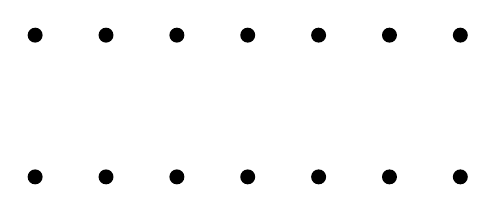
\begin{tikzpicture}[scale=.9]
  \foreach \x in {-3,...,3}
  \foreach \y in {-1,1}
  \fill (\x,\y) circle (3pt);
 \end{tikzpicture}
\end{center}

  \begin{answer}
    ${7\choose 2}{7\choose 2}$.
  \end{answer}



\question How many of the quadrilaterals possible in the previous problem are:

\begin{parts}
 \part Squares?
 \part Rectangles?
 \part Parallelograms?
 \part Trapezoids?\footnote{Here, as in calculus, a trapezoid is defined as a quadrilateral with \emph{at least} one pair of parallel sides.  In particular, parallelograms are trapezoids.}
 \part Trapezoids that are not parallelograms?
\end{parts}


  \begin{answer}
    \begin{parts}
      \part 5 (you need to skip one dot on the top and on the bottom). %Squares?
      \part ${7 \choose 2}$.  Once you select the two dots on the top, the bottom two are determined. % Rectangles?
      \part This is tricky since you need to worry about running out of space.  One way to count: break into cases by the location of the top left corner.  You get ${7 \choose 2} + ({7 \choose 2}-1) + ({7 \choose 2} - 3) + ({7 \choose 2} - 6) + ({7 \choose 2} - 10) + ({7 \choose 2} - 15)$. %Parallelograms?
      \part All of them %Trapezoids?
      \part All of them, except the parallelograms.  So ${7\choose 2}{7\choose 2} - \left[ {7 \choose 2} + ({7 \choose 2}-1) + ({7 \choose 2} - 3) + ({7 \choose 2} - 6) + ({7 \choose 2} - 10) + ({7 \choose 2} - 15) \right]$.
    \end{parts}
  \end{answer}




\question An \emph{anagram} of a word is just a rearrangement of its letters.  How many different anagrams of ``uncopyrightable'' are there?  (This happens to be the longest common English word without any repeated letters.)

	\begin{answer}
		Since there are 15 different letters, we have 15 choices for the first letter, 14 for the next, and so on.  Thus there are $15!$ anagrams.
	\end{answer}



\question How many anagrams are there of the word ``assesses'' that start with the letter ``a''?

	\begin{answer}
	 After the first letter, we must rearrange the remaining 7 letters.  There are only two letters, so this is really just a bit-string question.  Thus there ${7 \choose 2}$ anagrams starting with ``a''.
	\end{answer}


\question How many anagrams are there of ``anagram''?

	\begin{answer}
		First, decide where to put the ``a''s.  There are 7 positions, and we must choose 3 of them to fill with an ``a''.  This can be done in ${7 \choose 3}$ ways.  The remaining 4 spots all get a different letter, so there are $4!$ ways to finish off the anagram.  This gives a total of ${7 \choose 3}\cdot 4!$ anagrams.  Strangely enough, this is 840, which is also equal to $P(7,4)$.  To get the answer that way, start by picking one of the 7 \emph{positions} to be filled by the ``n'', one of the remaining 6 positions to be filled by the ``g'', one of the remaining 5 positions to be filled by the ``r'', one of the remaining 4 positions to be filled by the ``m'' and then put ``a''s in the remaining 3 positions.
	\end{answer}



\question On a business retreat, your company of 20 businessmen and businesswomen go golfing.
\begin{parts}
 \part You need to divide up into foursomes (groups of 4 people): a first foursome, a second foursome, and so on.  How many ways can you do this?
 \part After all your hard work, you realize that in fact, you want each foursome to include one of the five Board members.  How many ways can you do this?
\end{parts}

  \begin{answer}
    \begin{parts}
      \part ${20 \choose 4}{16 \choose 4}{12 \choose 4}{8 \choose 4}{4 \choose 4}$. %You need to divide up into foursomes (groups of 4 people): a first foursome, a second foursome, and so on.  How many ways can you do this?
      \part $5!{15 \choose 3}{12 \choose 3}{9 \choose 3}{6 \choose 3}{3 \choose 3}$. %After all your hard work, you realize that in fact, you want each foursome to include one of the five CEO's.  How many ways can you do this?
    \end{parts}
  \end{answer}



\question How many different seating arrangements are possible for King Arthur and his 9 knights around their round table?

  \begin{answer}
     $9!$ (there are 10 people seated around the table, but it does not matter where King Arthur sits, only who sits to his left, two seats to his left, and so on).
  \end{answer}



\end{questions}
